\documentclass[letterpaper]{article}  
\usepackage{graphicx}
\usepackage{float}
\usepackage[margin=1in]{geometry}
\usepackage{caption}
\usepackage{subcaption}
\usepackage{amsmath}
\usepackage{mathtools}
\usepackage{multicol}
\usepackage{dsfont}
\newcommand\myeq{\stackrel{\mathclap{\normalfont\mbox{set}}}{=}}

\usepackage{Sweave}
\begin{document}
\Sconcordance{concordance:hw6-sweave.tex:hw6-sweave.Rnw:%
1 12 1 1 0 432 1}


\begin{titlepage}
\title{\vspace{30mm}STA511 Final Homework}
\date{December 14, 2015}
\author{Abbas Rizvi}
\clearpage\maketitle
\thispagestyle{empty}
\end{titlepage}

\newpage
\section{Solutions}
\begin{enumerate}
\item Random normal variables were generated using the Laplace distribution given by:
$$g(x) = \frac{\theta}{2}e^{-\theta \vert x \vert} \text{, for } \theta > 0$$
\begin{enumerate}
\item The optimal rejection constant $c$ is $\texttt{1.315}$ and the optimal $\theta$ is $\texttt{1.0001}$ when $c = sup\frac{f(x)}{g(x)}$ where $f(x)$ is the standard normal pdf $\sim N(0,1)$. 

\begin{align*}
c =& sup\frac{f(x)}{g(x)}\\
c =& sup\Bigg(\frac{\frac{1}{\sqrt{2}\pi}e^{-x^{2}/2}}{\frac{\theta}{2}e^{-\theta\vert x \vert}}\Bigg)\\
c =& \frac{\sqrt{\frac{2}{\pi}}e^{\frac{-x^{2}}{2} - \theta \vert x \vert}}{\theta}\\
c =&
\begin{cases}
\frac{\sqrt{\frac{2}{\pi}}e^{\frac{-x^{2}}{2} + \theta x }}{\theta}, & \text{x } \geq 0  \\
\frac{\sqrt{\frac{2}{\pi}}e^{\frac{-x^{2}}{2} - \theta x }}{\theta}, & \text{x } < 0
\end{cases}
\end{align*}

Now we take the derivative of the upper piecewise function with respect to x. Afterwards we set the derivative to zero and solve for $\theta$.


\begin{align*}
c =& \frac{\sqrt{\frac{2}{\pi}}}{\theta} \Bigg[ e^{\frac{-x^{2}}{2} + \theta x} \frac{d}{dx}\Bigg] \\
  =& \frac{\sqrt{\frac{2}{\pi}}e^{\frac{-x^{2}}{2} + \theta x} \cdot (- x + \theta)}{\theta} = 0 \\
  \theta =& x \text{, for } x \geq 0
\end{align*}


Now we take the derivative of the lower piecewise function with respect to x. Afterwards we set the derivative to zero and solve for $\theta$.


\begin{align*}
c =& \frac{\sqrt{\frac{2}{\pi}}}{\theta} \Bigg[ e^{\frac{-x^{2}}{2} - \theta x} \frac{d}{dx}\Bigg] \\
   = & \frac{\sqrt{\frac{2}{\pi}}e^{\frac{-x^{2}}{2} - \theta x} \cdot (-x - \theta)}{\theta} = 0 \\
  \theta =& -x \text{, for } x < 0
\end{align*}

Each critical point was subsequently plugged into $c_{\theta}$ and both yielded the following:
$$ c = \frac{\sqrt{\frac{2}{\pi}}e^{\frac{\theta^{2}}{2}}}{\theta} \text{ , for} -\infty < 0 < \infty \text{ and } \theta > 0$$

The optimal $\theta$ was determined by minimzing the $c \geq \frac{f(x)}{g(x)}$ curve with respect to $\theta$. The function was computed with random variables and a corresponding plot was produced in \texttt{R} (Figure 1). The minimum $c$ ($\texttt{1.315489}$) and  optimal $\theta$ ($\texttt{1.0001}$) were computed using $\texttt{R}$'s $\texttt{nlminb}$ function. 

\begin{figure}[t]
\centering
\caption{}
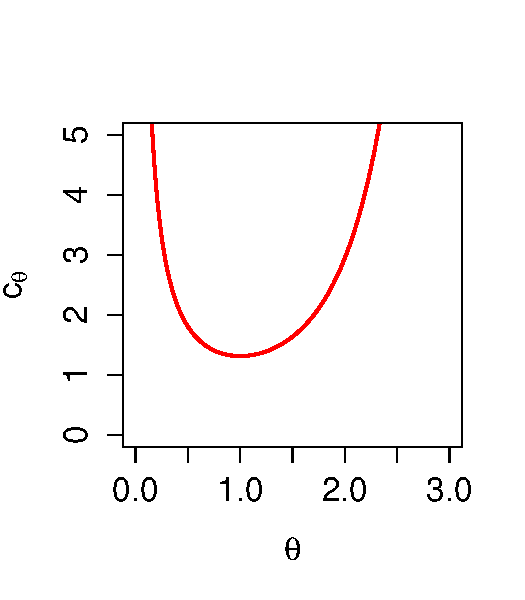
\includegraphics[width=2in]{/Users/aarizvi/Desktop/ROSWELL_PHD/STA511_StatisticalComputing/HW6/hw6-q1a.pdf}
\end{figure}

\item 1000 observations were generated from $N(0,1)$ using a generalized rejection method. In order to generate these observations, we have to sample from the Laplace distribution pdf g(x). Since we are sampling from a continuous distribution, in order to sample from the pdf, we need to first use the inversion method. The inversion method takes the quantile function of Laplace CDF G(x) to generate random variables of the Laplace pdf. The random variables then were sampled using the generalized rejection method, with \texttt{0.752} or 75.2\% of the observed random variables being accepted.

\begin{figure}
    \centering
    \caption{}
    \begin{subfigure}{0.4\textwidth}
        \centering
        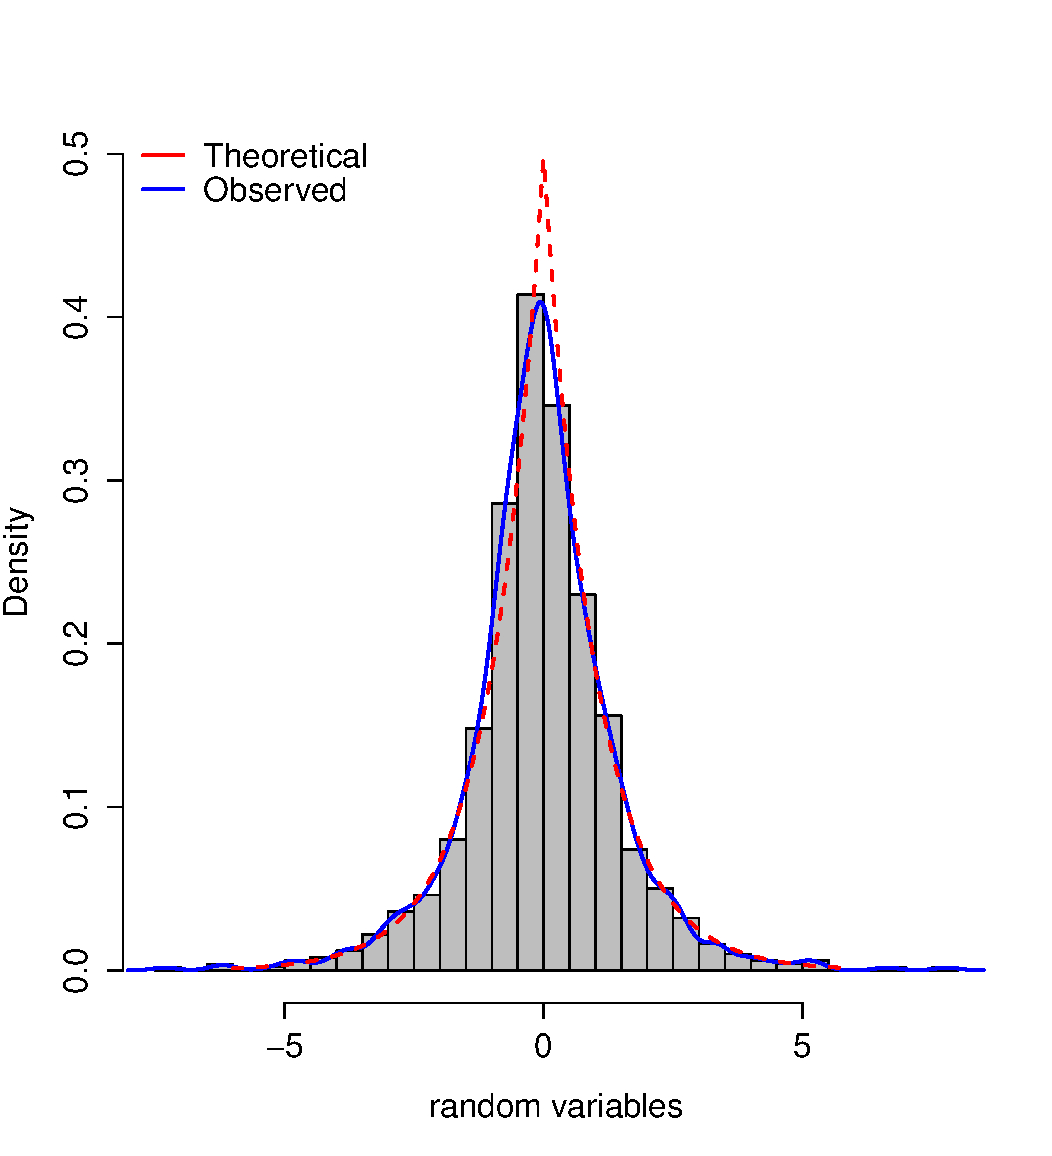
\includegraphics[width=\textwidth]{/Users/aarizvi/Desktop/ROSWELL_PHD/STA511_StatisticalComputing/HW6/hw6-q1b-1.pdf}
        \caption{Inversion Method}
    \end{subfigure}
    \begin{subfigure}{0.4\textwidth}
        \centering
        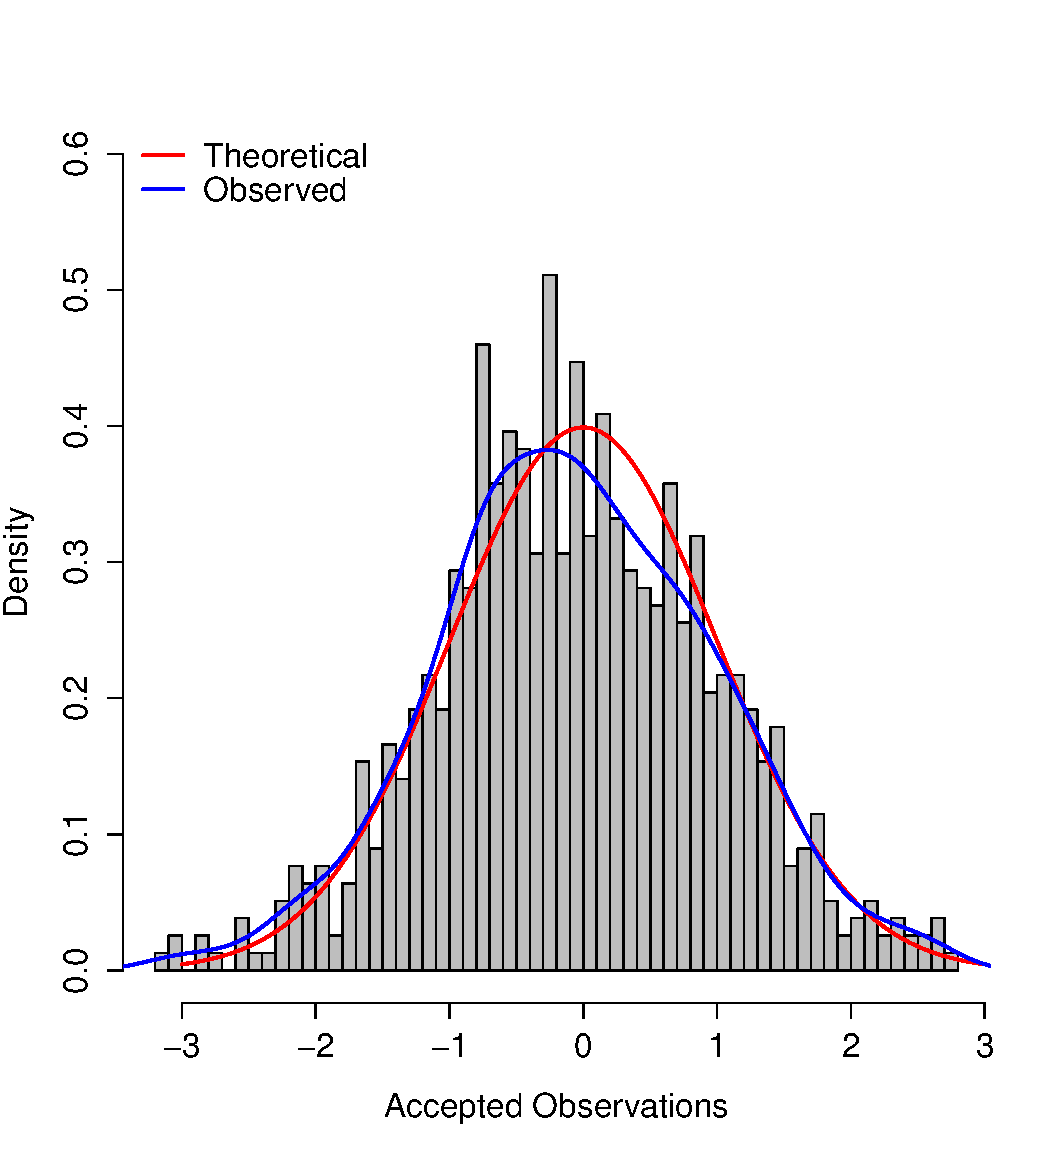
\includegraphics[width=\textwidth]{/Users/aarizvi/Desktop/ROSWELL_PHD/STA511_StatisticalComputing/HW6/hw6-q1b-2.pdf} 
        \caption{Generalized Rejection Method}
    \end{subfigure}
\end{figure}

$$
G(x) =
\begin{cases}
\frac{1}{2}e^{x} & x < 0\\
1- \frac{1}{2}e^{-x} & x \geq 0
\end{cases}
$$

$$
G^{-1}(p) =
\begin{cases}
ln(2p) & p \in [0, \frac{1}{2}]\\
-ln[2(1-p)] & p \in [\frac{1}{2},1]
\end{cases}
$$


\item A goodness of fit (Kolmogorov-Smirnov) test was conducted on the 1000 generated samples were consistent with a standard Normal Distribution. The null hypothesis for the K-S test is that the accepted (observed) Laplace random variables from the generalized rejection method were drawn from a normal distribution. The K-S test has a p-value of \texttt{0.43}, suggesting that we failed to reject the null hypothesis, colloquially meaning, that the Laplace random variables are likely to have been drawn from a standard normal distribution. This can be seen visually in Figure 2b. 
\end{enumerate}

\item I elected not to do problem 2.
\item The distribution described by the following density function was considered:
$$
f(x) =
\begin{cases}
x+1 & x \in [-1, 0]\\
-x+1 & x \in [0,1]\\
0 & \text{elsewhere}
\end{cases}
$$
\begin{enumerate}
\item The rejection method requires that pdf $f$ be bounded and nonzero only on some finite interval $[a,b]$. The rejection constant ($c$) was determined by $c = max\left\{f(x); a \leq x \leq b \right\}$. The following algorithm was implemented via \texttt{R}: \\

\begin{align*}
\text{1.}&  \text{ Generating } X \text{uniform on } (a,b).\\
\text{2.}& \text{ Generating } Y \text{uniform on } (0,c).\\
\text{3.}& \text{ If Y} \leq f(x), \text{then output} X, \text{otherwise go to } 1.
\end{align*}

100 random observations were generated from $f$ using simple rejection sampling. The accepted observations were \texttt{0.59} normalized to total number of generated observations. 

\item The inversion method involves sampling the PDF using the quantile of its CDF. We determined the CDF of the density function and then subsequently computed its corresponding quantile function. Since this given density follows a triangular distribution,  the CDF and quantile function are shown as:

$$
F(x) =
\begin{cases}
\frac{(x+1)^{2}}{2} & \text{for } -1 < x \leq 0\\
1 - \frac{(-x+1)^{2}}{2} & \text{for } 0 < x < 1 \\
\end{cases}
$$

$$
F^{-1}(u) =
\begin{cases}
\sqrt{2u}-1 & u \in [0,\frac{1}{2}]\\
1-\sqrt{2(-u+1)}& u \in [\frac{1}{2},1]
\end{cases}
$$


\item The histograms for part (a) and part (b) can be visualized in Figure 3a and Figure 3b, respectively.
\begin{figure}
    \centering
    \caption{}
    \begin{subfigure}{0.4\textwidth}
        \centering
        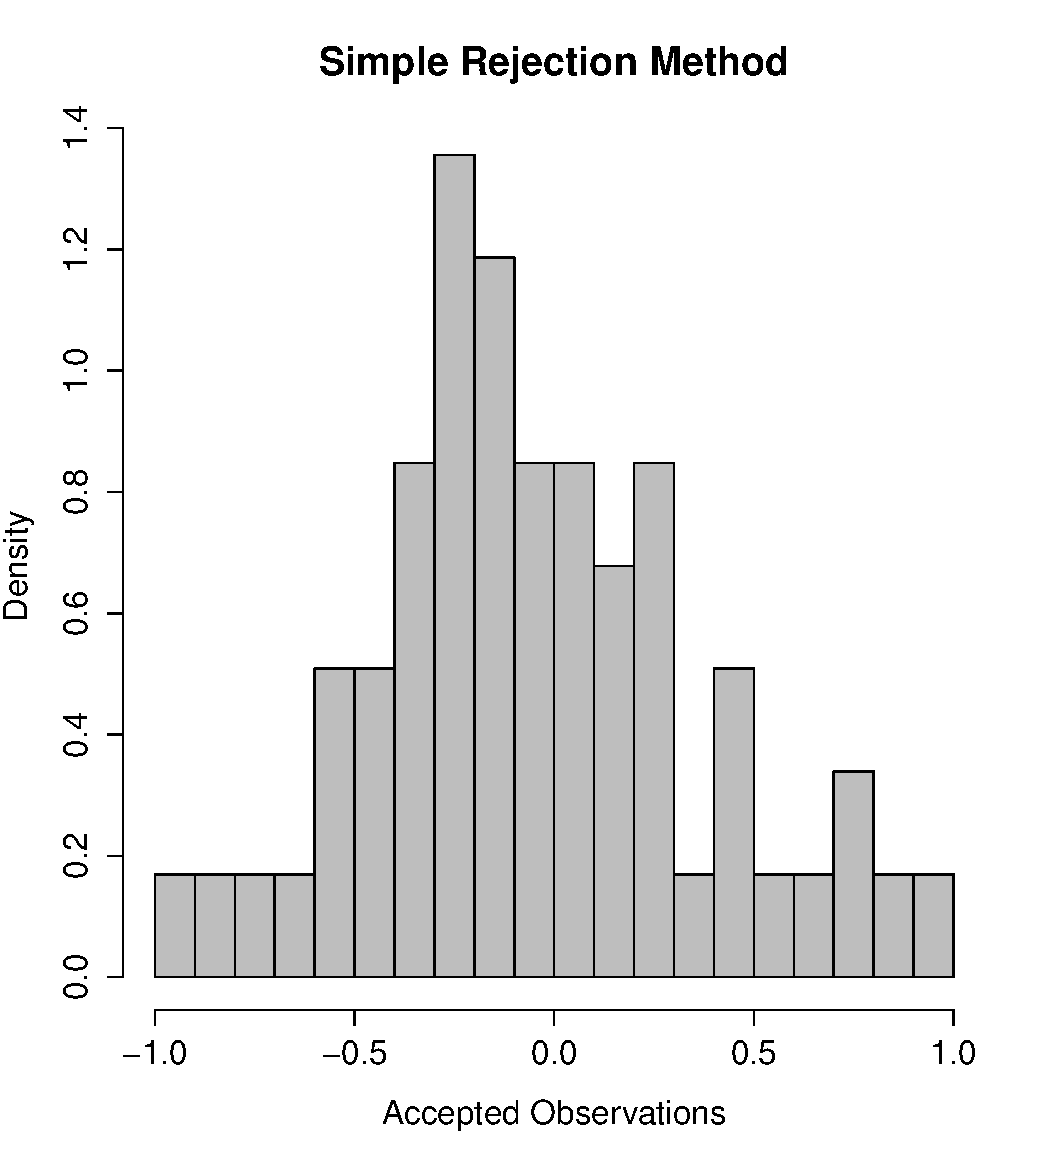
\includegraphics[width=\textwidth]{/Users/aarizvi/Desktop/ROSWELL_PHD/STA511_StatisticalComputing/HW6/hw6-q3c-1.pdf}
        \caption{Simple Rejection Method}
    \end{subfigure}
    \begin{subfigure}{0.4\textwidth}
        \centering
        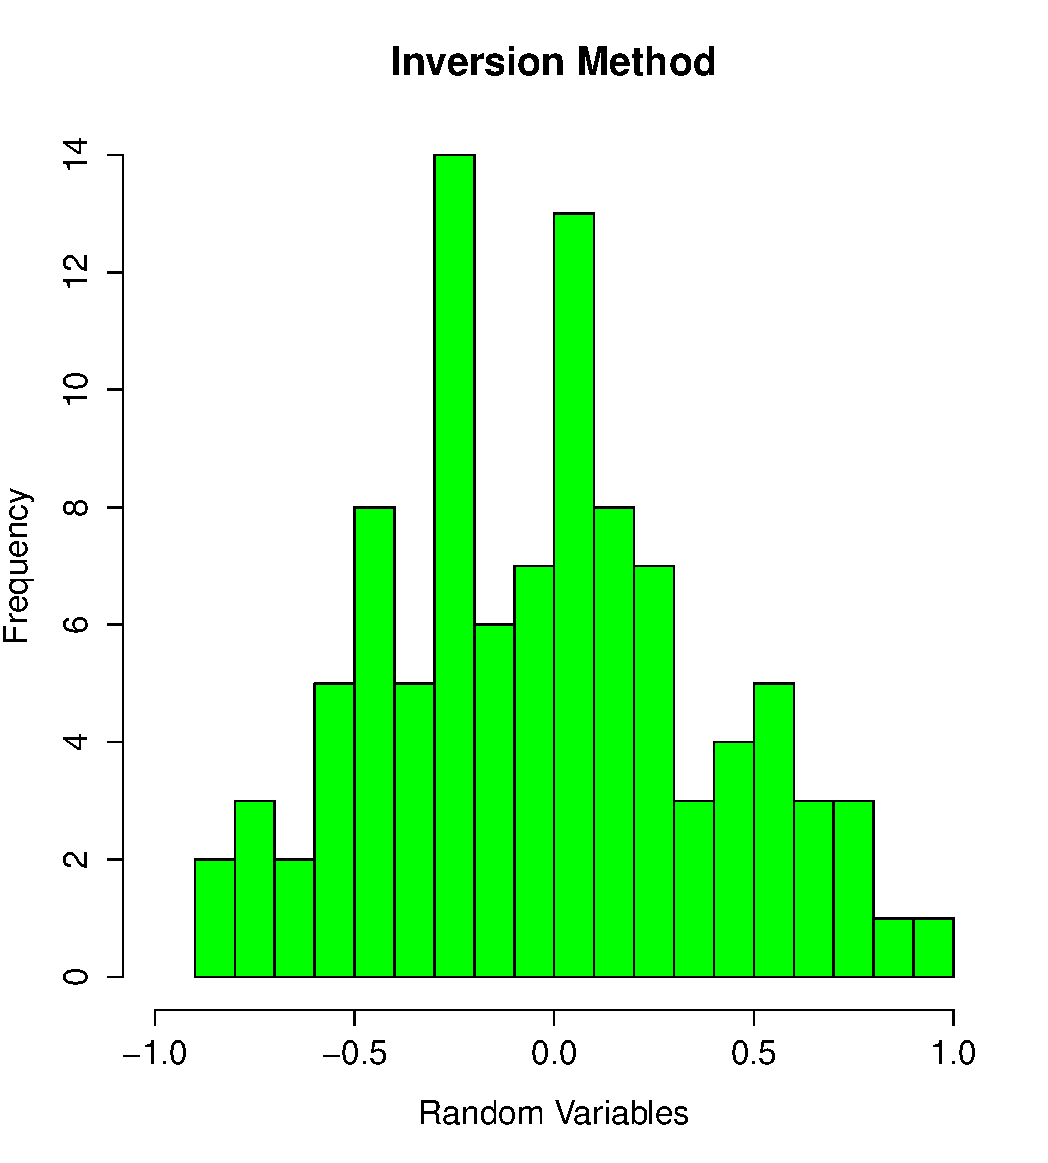
\includegraphics[width=\textwidth]{/Users/aarizvi/Desktop/ROSWELL_PHD/STA511_StatisticalComputing/HW6/hw6-q3c-2.pdf} 
        \caption{Inversion Method}
    \end{subfigure}
\end{figure}



\end{enumerate}

%Question 4
\item Simulations were conducted such that a coin was flipped until a pattern emerged. Pattern 1 was given as head (H), tail (T), tail (T), and pattern 2 was head (H), tail (T), head (T). The first simulation was the average number of tosses needed to obtain pattern 1 or pattern 2. The second simulation simulated 100,000 flips and counted the number occurrences of pattern 1 and 2.
\begin{enumerate}
\item 1,000 iterations were conducted for the first simulation. The average number of flips needed until pattern 1 (HTT) emerged was $\texttt{7.138}$. The average number of flips needed until pattern 2 (HTH) emerged was $\texttt{9.491}$. This answer does not surprise me. Intuitively, pattern 1 should occur in fewer flips because after 2 flips if the pattern is H-T,  if a tail emerges as the subsequent flip in the sequence, the desired pattern (pattern 1) has been reached, but if heads emerges, the pattern is not penalized as much as pattern 2 (HTH) because H is the first flip (position 1) needed for pattern 1. However, on the contrary, if the sequence of flips was already H-T, pattern 2 would be achieved with a 3rd flip of H, but if it is T, the flips continue until a H is achieved to start the desire pattern again.

\item A simulation with 10 iterations was conducted in order to count how many times pattern 1 and pattern 2 emerged in 100,000 flips. Pattern 1 emerged 12540/100000 flips (12.54\%) and pattern 2 emerged 12472/100000 flips (12.47\%). These values are quite close, with pattern 1 still occuring more often. I thnk that these results more or less agree with part (a) because the probability of each outcome per flip is 0.5, so with such a large sample population, I would expect the number of occurrences to be close to one another, with a slight edge towards the more likely pattern (pattern 1). 
\end{enumerate}
\item Let $X_{1},...,X_{n}$ $\sim$ Uniform($a$,5) where $a$ is an unknown parameter.
\begin{enumerate}
\item The methods of moments estimator for $a$ was found to be:
\begin{align*}
E[X] =& \bar{X}\\
\frac{a-5}{2} =& \sum^{n}_{i=1}{\frac{X_{i}}{n}}\\
\tilde{a}_{MOM} =& \frac{2\sum^{n}_{i=1}{X_{i}}}{n} - 5
\end{align*}

\item The MLE for $\alpha$ was found to be:
\begin{align*}
MLE =& (\hat{a}, \hat{b}) = (\text{min}\left\{X_{[1]}\right\},\text{max}\left\{X_{[n]}\right\})\\
L(X_{i}|a) =& \prod^{n}_{i=1} \Bigg[ \frac{1}{5-\alpha}\Bigg]^{n} \text{, for } \alpha \leq x \leq 5\\
=& \Bigg[ \frac{1}{5-a} \Bigg]^{n} \text{, for } \alpha \leq \text{min}\left\{X_{[i]}\right\} \leq \text{max}\left\{X_{[n]}\right\} \leq 5\\
\hat{a}_{MLE} =& X_{[1]} 
\end{align*}

\item $\tau = E(X) = \int^{5}_{a} x \cdot f(x)dx$ where $f(x) = \frac{1}{5-a}$. The MLE for $\tau$ was found to be:

\begin{align*}
\tau = E(X) =& \int^{5}_{a} x \cdot f(x) dx \\
=& \int^{5}_{a} x \cdot \frac{1}{5-a} dx\\
=& \frac{1}{5-a} \int^{5}_{a} x dx \\
=& \frac{1}{5-a} \Bigg[ \frac{x^{2}}{2} \Bigg\vert^{5}_{a} \Bigg]\\
=& \frac{1}{5-a} \Bigg(\frac{5^{2} - a^{2} } {2} \Bigg)\\
=& \frac{1}{5-a} \Bigg(\frac{(5-a)(5+a)} {2} \Bigg)\\
\hat{\tau}_{MLE} =& \frac{5+\hat{a}_{MLE}}{2}
\end{align*}

\item Let $\hat{\tau}$ be the MLE of $\tau$. Let $\tilde{\tau}$ be the MOM based estimator of $\tau = E(X)$.
\begin{align*}
\hat{\tau}_{MLE} =& \frac{5+X_{[1]}}{2}\\
\tilde{\tau}_{MOM} =& \frac{5+2\sum^{n}_{i=1}{X_{i}}}{2n}
\end{align*}

We suppose that $a = 1$ and $n = 10$. 

$$\bar{X} = \frac{\sum^{n=10}_{i=1}{X_{i}}}{n}$$

The coverage probability was computed for a 95\% confidence interval for $\tau$ bootstrap method with $\hat{\tau}$. The confidence intervals were:

\begin{align*}
\text{Normal CI: }& (2.83,3.24)\\
\text{Pivotal CI: }& (2.47,3.04)\\
\text{Percentile CI: }& (3.04, 3.61)
\end{align*}
This was compared to the coverage prbability for a 95\% interval for $\tau$ using the same bootstrap method but for $\tilde{\tau}$ instead of $\hat{\tau}$. The confidence intervals were:

\begin{align*}
\text{Normal CI: }& (1.90,3.39)\\
\text{Pivotal CI: }& (1.90,3.36)\\
\text{Percentile CI: }& (1.94, 3.39)
\end{align*}

\end{enumerate}

\end{enumerate}
\newpage

\section{Appendix}
\begin{enumerate}
\item 
\begin{verbatim}
#part a
foverg <- function(theta){sqrt(2/pi)*exp(theta^2/2)/theta}

theta <- seq(0.000001, 10, length=1000)

opt.theta <-nlminb(0.00001,function(theta){foverg(theta)})$par
c <- nlminb(0.00001,function(theta){foverg(theta)})$objective

plot(theta,(sqrt(2/pi)*exp(theta^2/2))/theta,type="l", col="red",lwd=2,ylim=c(0,5),xlim=c(0,3), 
     ylab=expression(c[theta]),xlab=expression(theta))

#part b
#inversion method
laplace.inv <- function(p){
       if(p < 1/2){
               log(2*p, base=exp(1))
       } else {
               -log(2*(1-p), base=exp(1))
       }
}

p <- runif(1000)
laplace.rv <- sapply(p,laplace.inv) #random variables from laplace
hist(laplace.rv)
laplace.dist <- function(x){ #theta as 1
        if(x<0){
                (1/2)*exp(x)
        }else {
                (1/2)*exp(-x)
        }
}

rvs <- seq(-6,6,length=1000)
laplace.pdf <- sapply(rvs,laplace.dist)
hist(laplace.rv, ylim=c(0,0.5), col="gray", xlab="random variables", prob=T, breaks=50, main="")
lines(density(laplace.rv), col="blue", lwd=2)
lines(rvs, laplace.pdf, col="red", lwd=2, lty=2)
legend("topright",legend=c("Theoretical PDF","Observed PDF"),
       col=c("red", "blue"),lwd=c(2,2), bty="n")

#generalized rejection method
goverf <- function(x,theta=1){y = sqrt(pi/2)*theta*exp((x^2/2)-theta*abs(x))}
xc <- laplace.rv
uc <- runif(1000,0,1)
tc <- c*sapply(xc,goverf)
ut <- uc*tc
accept.obs <- xc[ut <= 1]
length(accept.obs)/1000

nseq <- seq(-3,3,length=1000)
norm <- dnorm(nseq)

hist(accept.obs, col="gray", prob=T, breaks=50, ylim=c(0,0.6), 
xlab = "Accepted Observations", main="")
lines(nseq, norm, col="red", lwd=2)
lines(density(accept.obs), col="blue", lwd=2)
legend("topright",legend=c("Theoretical PDF","Observed PDF"),
       col=c("red", "blue"),lwd=c(2,2), bty="n")
       

#part c
ks.test(accept.obs, "pnorm", 0,1)

        One-sample Kolmogorov-Smirnov test

data:  accept.obs
D = 0.0319, p-value = 0.43
alternative hypothesis: two-sided
\end{verbatim}

\item Did not do question 2.
\item 
\begin{verbatim}
####question 3####
#part a
rm(list=ls())
set.seed(333)
f.pdf <- function(x){
        if(-1 <= x & x <= 0){
                x + 1
        }else if(0 <= x & x <= 1){
                -x + 1
        }
        else{
                0
        }
}
c.max <- optimize(f.pdf, interval=c(-1,1), maximum=TRUE)$objective
#simple rejection
xc <- runif(100,-1,1) #generate x uniform[a,b]
uc <- runif(100,0,1) #generate uniform [0,1]
tc <- c.max/sapply(xc,f.pdf) #t = c/fx
ut <- uc*tc
accept.obs <- xc[ut <= 1]
length(accept.obs)/100 #accept 50.6%


#part b
#inversion method
icdf <- function(u){   
        if(0 < u & u < 0.5){
                sqrt(2*u)-1
        }else if(0.5 <= u & u < 1){
                1 - sqrt(2*(-u+1))
        }else{
                u=0}
}
rand.unif <- runif(100,0,1)
rvs <- sapply(rand.unif, icdf)
hist(rvs, col="green", breaks=20, main="Inversion Method", xlab="Random Variables", xlim=c(-1,1))

#part c is in a and b
\end{verbatim}
\item 
\begin{verbatim}
#part a
rm(list=ls())
require(zoo)
set.seed(333)
coinflip <- function(seq){
        flip <- c()
        ht <- c()
        match <- FALSE
        while (any(match) == FALSE){
                flip <- sample(c("H", "T"), 1, replace = TRUE, prob=c(0.5,0.5))
                ht <- c(ht,flip)
                if (length(ht) > 3){
                        match <- rollapply(ht,3,identical,seq)
                }
        }
        return(length(match)+1)
}

num.trials <- 1000
trials <- data.frame("hth"=rep(NA,num.trials),"htt"=rep(NA,num.trials))
for (i in 1:num.trials){
        trials[i,] <- c(coinflip(c("H","T","H")), coinflip(c("H","T","T")))
}
summary(trials)

      hth              htt        
 Min.   : 3.000   Min.   : 3.000  
 1st Qu.: 4.000   1st Qu.: 3.000  
 Median : 7.000   Median : 6.000  
 Mean   : 9.491   Mean   : 7.138  
 3rd Qu.:13.000   3rd Qu.: 9.000  
 Max.   :59.000   Max.   :47.000

#part b
rm(list=ls())
set.seed(333)
require(zoo)
num.trials <- 10
trials <- data.frame("hth"=rep(NA,num.trials),"htt"=rep(NA,num.trials))
for (j in 1:num.trials){
        coin <- c('h','t')
        s <- sample(x=coin, size=100000, replace=T, prob=c(0.5,0.5))       
        hth <- length(which(rollapply(s,3,identical,c("h","t","h"))))
        htt <- length(which(rollapply(s,3,identical,c("h","t","t"))))
        trials[j,] <- c(hth,htt)
}
>summary(trials)
      hth             htt       
 Min.   :12292   Min.   :12447  
 1st Qu.:12436   1st Qu.:12509  
 Median :12472   Median :12548  
 Mean   :12478   Mean   :12540  
 3rd Qu.:12553   3rd Qu.:12570  
 Max.   :12587   Max.   :12625
\end{verbatim}

\item 
\begin{verbatim}
##########################
####### question 5D ######
##########################
rm(list=ls())
set.seed(333)
x.i <- runif(10,1,5)
tau.mle <- (5+min(x.i))/2
tau.mom <- mean(x.i)
t.mle <- c()
t.mom <- c()
for(i in 1:10000){
        boot.obs <- sample(x.i, 10, replace = T)
        t.mle[i] <- (5+min(boot.obs))/2
        t.mom[i] <- mean(boot.obs)
}
se.mle = sqrt(var(t.mle))
se.mom <- sqrt(var(t.mom))

Normal.mle = c(tau.mle-2*se.mle, tau.mle+2*se.mle)
Normal.mom = c(tau.mom-2*se.mom, tau.mom+2*se.mom)

pivotal.mle = c(2*tau.mle-quantile(t.mle,.975),2*tau.mle-quantile(t.mle,.025))
pivotal.mom = c(2*tau.mom-quantile(t.mom,.975),2*tau.mom-quantile(t.mom,.025))

percentile.mle <- c(quantile(t.mle,0.025),quantile(t.mle,0.975))
percentile.mom <- c(quantile(t.mom,0.025),quantile(t.mom,0.975))
\end{verbatim}

\end{enumerate}



\end{document}
